% Source: graduate-coursework/Research/Intro_to_Agents/handouts/Part7_Parallelization.tex

\documentclass[border=4pt]{standalone}
\usepackage{amsmath,amssymb,amsfonts}
\usepackage[T1]{fontenc}
\usepackage{graphicx}
\usepackage{lmodern}
\usepackage{tikz}
\usepackage{xcolor}
\usetikzlibrary{shapes.geometric, arrows.meta, positioning, calc, fit, backgrounds, matrix, decorations.pathreplacing}

\definecolor{UofSCGarnet}{HTML}{73000a}
\definecolor{UofSCBlack}{HTML}{000000}
\definecolor{UofSCWhite}{HTML}{ffffff}
\definecolor{UofSCRose}{HTML}{CC2E40}
\definecolor{UofSCAtlantic}{HTML}{466A9F}
\definecolor{UofSCCongaree}{HTML}{1F414D}
\definecolor{UofSCHorseshoe}{HTML}{65780B}
\definecolor{UofSCGrass}{HTML}{CED318}
\definecolor{UofSCHoneycomb}{HTML}{A49137}
\definecolor{UofSC90Black}{HTML}{363636}
\definecolor{UofSC70Black}{HTML}{5C5C5C}
\definecolor{UofSC50Black}{HTML}{A2A2A2}
\definecolor{UofSCWarmGrey}{HTML}{676156}
\definecolor{UofSCSandstorm}{HTML}{FFF2E3}
\definecolor{UofSCDarkGarnet}{HTML}{570008}
\definecolor{UofSCAzalea}{HTML}{844247}

\tikzset{
    % Node styles - all with sharp corners
    agentbox/.style={
        rectangle,
        draw=UofSCGarnet,
        fill=UofSCSandstorm,
        thick,
        minimum width=2cm,
        minimum height=0.8cm,
        text centered,
        font=\footnotesize
    },
    processbox/.style={
        rectangle,
        draw=UofSCAtlantic,
        fill=UofSCWhite,
        thick,
        minimum width=2.5cm,
        minimum height=0.7cm,
        text centered,
        font=\footnotesize
    },
    syncbox/.style={
        rectangle,
        draw=UofSCCongaree,
        fill=UofSCCongaree!20,
        thick,
        minimum width=3cm,
        minimum height=0.5cm,
        text centered,
        font=\footnotesize\bfseries
    },
    resultbox/.style={
        rectangle,
        draw=UofSCHorseshoe,
        fill=UofSCGrass!30,
        thick,
        minimum width=2cm,
        minimum height=0.7cm,
        text centered,
        font=\footnotesize
    },
    % Arrow styles
    myarrow/.style={
        ->,
        >=Stealth,
        thick,
        UofSCBlack
    },
    dashedarrow/.style={
        ->,
        >=Stealth,
        thick,
        dashed,
        UofSC70Black
    },
    % Timeline styles
    timeline/.style={
        draw=UofSCBlack,
        thick,
        ->,
        >=Stealth
    },
    timeblock/.style={
        rectangle,
        draw=none,
        minimum height=0.5cm,
        text centered,
        font=\tiny
    }
}

\begin{document}
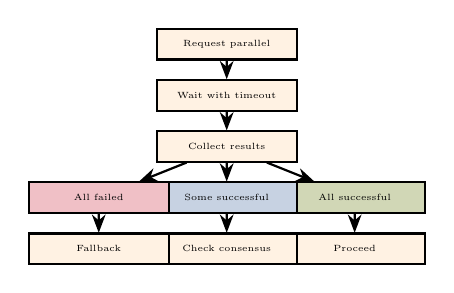
\begin{tikzpicture}[scale=0.65, transform shape,
                stepbox/.style={rectangle, draw=UofSCBlack, thick, fill=UofSCSandstorm, text width=2.5cm, text centered, font=\tiny, minimum height=0.6cm}
            ]
                \node[stepbox] (req) at (0,4) {Request parallel};
                \node[stepbox] (wait) at (0,3) {Wait with timeout};
                \node[stepbox] (collect) at (0,2) {Collect results};

                \node[stepbox,fill=UofSCHorseshoe!30] (allsuc) at (2.5,1) {All successful};
                \node[stepbox,fill=UofSCAtlantic!30] (some) at (0,1) {Some successful};
                \node[stepbox,fill=UofSCRose!30] (allfail) at (-2.5,1) {All failed};

                \node[stepbox] (proceed) at (2.5,0) {Proceed};
                \node[stepbox] (consensus) at (0,0) {Check consensus};
                \node[stepbox] (fallback) at (-2.5,0) {Fallback};

                \draw[myarrow] (req) -- (wait);
                \draw[myarrow] (wait) -- (collect);
                \draw[myarrow] (collect) -- (allsuc);
                \draw[myarrow] (collect) -- (some);
                \draw[myarrow] (collect) -- (allfail);
                \draw[myarrow] (allsuc) -- (proceed);
                \draw[myarrow] (some) -- (consensus);
                \draw[myarrow] (allfail) -- (fallback);
            \end{tikzpicture}
\end{document}
